% Straight up stealing preamble from Eli Holmes 
%%%%%%%%%%%%%%%%%%%%%%%%%%%%%%%%%%%%%%START PREAMBLE THAT IS THE SAME FOR ALL EXAMPLES
\documentclass{article}

%Required: You must have these
\usepackage{Sweave}
\usepackage{graphicx}
\usepackage{tabularx}
\usepackage{hyperref}
\usepackage{natbib}
\usepackage{pdflscape}
\usepackage{array}
\usepackage{gensymb}
%\usepackage[backend=bibtex]{biblatex}
%Strongly recommended
  %put your figures in one place
%\SweaveOpts{prefix.string=figures/, eps=FALSE} 
%you'll want these for pretty captioning
\usepackage[small]{caption}

\setkeys{Gin}{width=0.8\textwidth}  %make the figs 50 perc textwidth
\setlength{\captionmargin}{30pt}
\setlength{\abovecaptionskip}{10pt}
\setlength{\belowcaptionskip}{10pt}
% manual for caption  http://www.dd.chalmers.se/latex/Docs/PDF/caption.pdf

%Optional: I like to muck with my margins and spacing in ways that LaTeX frowns on
%Here's how to do that
 \topmargin -1.5cm        
 \oddsidemargin -0.04cm   
 \evensidemargin -0.04cm  % same as oddsidemargin but for left-hand pages
 \textwidth 16.59cm
 \textheight 21.94cm 
 %\pagestyle{empty}       % Uncomment if don't want page numbers
 \parskip 7.2pt           % sets spacing between paragraphs
 %\renewcommand{\baselinestretch}{1.5} 	% Uncomment for 1.5 spacing between lines
\parindent 0pt% sets leading space for paragraphs
\usepackage{setspace}
%\doublespacing

%Optional: I like fancy headers
%\usepackage{fancyhdr}
%\pagestyle{fancy}
%\fancyhead[LO]{How do climate change experiments actually change climate}
%\fancyhead[RO]{2016}
 
%%%%%%%%%%%%%%%%%%%%%%%%%%%%%%%%%%%%%%END PREAMBLE THAT IS THE SAME FOR ALL EXAMPLES

%Start of the document
\begin{document}

%\SweaveOpts{concordance=TRUE}
\bibliographystyle{..//..//refs/bibstyles/amnat.bst}% i moved a style file into the ospree git repo. feel free to add whatever style you like and update, lizzie! I don't have besjournals

\title{Chilling outweighs photoperiod and forcing cues for temperate trees in experiments, but not in natural systems} % perspective paper for OSPREE analyses
% or Chilling dominates tree budburst in controlled climate experiments, but not in the great outdoors

\author{A.K. Ettinger, C. Chamberlain, I. Morales-Castilla, D. Buonaiuto, D. Flynn, T. Savas, \\J. Samaha \& E. Wolkovich}
%\date{\today} 
\maketitle  %put the fancy title on
%\tableofcontents      %add a table of contents
%\clearpage
%%%%%%%%%%%%%%%%%%%%%%%%%%%%%%%%%%%%%%%%%%%%%%%%%%%

% To do:
% Intro is 2-3X too long, we should clean it up, save it for a longer version of the ms in case we need it, then cut it down.
% The two paragraphs on chilling followed by the one on interactions should be *at least halved* once we have the rest of the text sorted. I also think they break up the flow so wonder if we could read them.
% Word count is about 2300, need to cut to 1500-1800 if possible (once happy).
% Think on: we say 'our model' a lot; we also say our findings, results or OSPREE ... we should be sure we like the language and keep it easy to follow (perhaps less 'our model' though I am not sure). 

% Smaller to do/questions etc.
% Flesh out all the methods (XX studies, species etc.) and results (more XX for Weinberger etc.).
% We say 'the forcing sensitivity in our model (-0.85 days per degree of warming) is consistent with what previous experiments and observational studies have observed (Wolkovich et al., 2012b; Menzel et al., 2006)' but is it? I think it is actually rather small (I think because it averages over interactions).  We can just CUT THIS I think...

%%%%%%%%%%%%%%%%%%%%%%%%%%%%%%%%%%%%%%%%%%%%%%%%%%%


\begin{abstract}
Decades of fundamental research on woody plant species highlight how three major cues shape spring phenological events: forcing (warm temperatures, generally occurring in the late winter and early spring), daylength, and chilling (cool temperatures, generally occurring in the fall and late winter). As research on the biological impacts of climate change has grown it has led to debate over whether forcing cues may dominate in nature for some or many species, while fewer respond to chilling and/or daylength. The debate has wide-reaching consequences for the future of spring phenology, as the presence of strong chilling or daylength cues could slow, stall, or even reverse current trends towards ever-earlier spring phenology with warming. Here we use a global meta-analysis of all published growth chamber studies to test for the relative effects of these three major cues across XX species. We find almost all species show strong responses to all three cues, with chilling being the strongest cue (numbers), followed by forcing (numbers) and daylength (numbers). Simple forecasts from our findings, however, suggest that the impact of chilling and daylength cues is highly location-specific---dependent largely on whether chilling increases or decreases with warming---and may not have a major impact on projections in well-studied areas (e.g., Central Europe) without warming of 4\degree C or more. Our results, thus, unify both sides of the debate over phenological cues: while all species may respond to all cues strongly in experimental conditions, in current environmental conditions the dominant impact of climate change is---and may remain---from increased forcing.  %The magnitude of future shifts in phenology depends largely . %not sure we're ready to say this last sentence yet...depends on forecasting with full set of PEP data.
% How pervasive these cues are and whether some species are effectively governed by only one or two cues is a critical area of climate change biology research, as it would shape how complex responses to warming will be. 
% These results suggest that future responses to warming will be complex. 
\end{abstract}

\section* {Text so far...}

\par For decades, plant phenology has been one of the most reported and consistent biological imprints of climate change \citep{IPCC:2014sm}, with many temperate plants leafing and flowering days to weeks earlier with rising temperatures \citep{millerrushing2008,menzel2006}. Understanding such shifts is important as phenology shapes a suite of ecosystem services, including pollination and carbon sequestration, and scales up to impact projections of climate change itself \cite{diez2012,richardson2013}. 

\par As research interest in phenology has progressed, critical discrepancies and uncertainties in our understanding have emerged. Though responses to warming are consistent on average, they show high unexplained variation across species and sites \citep{Wolkovich:2012n}. Furthermore, long-term observational studies provide increasing evidence that sensitivities of phenology to temperature are weakening in recent decades \cite{Rutishauser:2008,yu2010}, especially in Europe, where researchers suggest that responses to environmental cues beyond forcing underlie declining temperature sensitivities  \cite{fu2015}.
%  In Europe, recent work from many of the most well-studied tree species shows declining responses to temperature, suggesting that the long-term trend towards ever-earlier springs may be stalling \citep{fu2015}.

\par Fundamental research in phenology outlines how three major cues,  chilling, forcing, and daylength, provide multiple routes to budburst each spring, depending on the environment \citep{chuineJTB}. For example, in some species a cool winter resulting in high chilling will require a lower amount of forcing to trigger budburst, compared to a warmer winter that results in significantly lower chilling \citep{harrington2015}. In other species daylength may help trigger budburst given low chilling and/or forcing \citep{Basler:2014aa, Caffarra:2011b, zohner2016}. Research suggests that all three cues may underlie spring phenology for many temperate woody species \citep{flynn2018,Basler:2014aa,Caffarra:2011qf}. However, there is strong debate, with some research suggesting some cues---such as photoperiod---may be effectively absent in some species, but dominate in others \citep{zohner2016,koerner2010a}. 

% Below and above ... do we really want to discuss thresholds and 'unfufilled cues' or can we get around it?
\par Resolving this debate requires overcoming major hurdles to estimate responses to each cue. While a number of studies have tried to do this using long-term observational data \citep{vitasse2013, zohner2016}, these studies generally fail to overcome the fundamental challenge that all three cues are strongly correlated in nature (e.g., during the transition from winter to spring at temperate latitudes, forcing and daylength usually increase in step). In contrast to observational studies, controlled environment experiments can break correlations between chilling, forcing. These experiments---most often conducted in growth chambers or similar systems to control temperature and light---have been conducted for decades. To date, however, they have identified contrasting effects of the three major cues \citep{zohner2016,Laube:2014a,Basler:2012,Caffarra:2011b,Caffarra:2011a}
% Some studies report that photoperiod is likely to constrain species responses to climatic warming \citep{Basler:2012, Caffarra:2011b,Caffarra:2011a}, whereas others state that photoperiod is not a strong cue \citep{zohner2016,Laube:2014a} and that chilling is more important to current and future trends. 
% Given the declining response to temperature observed in long-term observational studies \citep{fu2015}, a number of studies have tried to tease out evidence that chilling or daylength cues are playing an increasingly important role in recent years \citep{Basler:2014aa,zohner2016, Laube:2014a}. This work must overcome the fundamental challenge that all three cues are strongly correlated in nature: e.g., during the transition from winter to spring at temperate latitudes, air temperatures increase (i.e., forcing increases) at the same time that daylength increases. 

% We could potentially cut the below.... may be repetitive with what we have above?
\par Resolving these discrepencies to identify which cues most strongly affect spring phenology is critical for forecasting future phenological changes. If forcing is the dominant cue (as many observational studies to date have assumed, \citep{bradley1999,menzel2006,harrington2015}), then we can expect additional spring advancement as temperatures continue to warm. However, if chilling limits budburst, then we may see delays in spring phenology as further global warming reduces chilling in many areas \citep{fraga2019}. 

% We should ONLY report the data that went into the budburst analysis. 
\par Here, we leverage nearly 40 years of controlled environment studies to understand how chilling, forcing, and photoperiod contribute to budburst timing in woody species. Using a meta-analytic approach we reviewed XX papers from controlled environment studies, then extracted data from any papers that reported budburst responses, yielding data from 74 studies across 39 years and 223 species (reference map of studies).  This database includes only studies for which we could identify forcing, photoperiod, and chilling treatments quantitatively. As chilling was rarely reported, we estimated chilling (when possible) using local climate data (see Supplemental Materials). We used a Bayesian hierarchical model to estimate the effects of chilling, forcing, and photoperiod. This model estimates both species-level responses (generally yielding more accurate estimates for well-studied species, such as \emph{Fagus sylvatica, Betula penndula}) and the distribution from which they are drawn, yielding a higher-level estimate of the overall response across species (see Supplemental Materials- mention species complex).\\ % 'Partial pooling' is too complex a term for most readers so I suggested we avoid it and move any greater discussion about the model to the supp where we can include an equation. 


\par Across studies, all cues---chilling, forcing, and photoperiod--- advance budburst phenology (Fig. \ref {fig:mu}). Using a standardized scale to allow comparisons of the three cues we found that chilling was the strongest cue (-2.86 days/standard unit or -8.87 days per 240 Utah units, which is typically about 10 days of chilling, Fig. \ref {fig:apc}), followed by forcing (-0.79 days/standard unit or -4.37 days per \degree C of warming, Fig. \ref {fig:apc}), and photoperiod (-0.53 days/standard unit or -3.13 days per hour of daylength). While photoperiod had the smallest effect among the three cues, our results contrast with the extensive literature suggesting photoperiod is a weak or non-existent cue for many species \citep{zohner2016,koerner2010a}---instead we found it was surprisingly large and consistent across species. Only \emph{Fagus sylvatica}, a species well-known for having a large response to photoperiod deviated far from the overall estimate (Figure \ref {fig:mu}). Species also showed fairly consistent responses to chilling (sigma = 2.06 days per 240 Utah units, Figure \ref {fig:mu}%, though two species delayed budburst with chilling \emph{Tilia codata}, \emph{Salix} complex)%only if chillportions used.
Responses to forcing, in contrast, were the most variable across species (sigma = 0.91 days per \degree C of warming).
% SIGMA needs a unit

% Is the below -- aside from the provenance stuff -- covered in the above (or previously in the intro)? I think so, in which case we can just look out for where to tuck the latitude finding in.
%  \par It has been proposed that photoperiod limitation may also reduce advancement rates of spring budburst for some species \citep{koerner2010a}. We find that photoperiod responses were consistent across species, suggesting that all species rely on this cue for spring phenology \citep{zohner2016, flynn2018,Caffarra:2011a}. Sensitivity to daylength may protect new plant tissues from frost damage by delaying budburst date until a lower risk time of year \citep{koerner2010a}. The magnitude of photoperiod sensitivity varied with provenance latitude: woody material from lower latitudes generally had earlier budburst, given the same chilling, forcing, and daylength conditions (cite supplemental table or figure showing latitude model). %Though we found widespread photoperiod sensitivity across species, the effect was small in comparison to forcing and chilling.

\par As temperature is radically altered by anthropogenic climate change, our finding that different ends of the temperature spectrum---chilling and forcing---have the strongest effects on budburst suggests that understanding these cues will be critical for forecasting. Many previous studies attribute advances in budburst to increased forcing \citep{Basler:2014aa,bradley1999,menzel2006,harrington2015}, and forcing sensitivity in our model (-4.37 days per degree of warming) is consistent with what previous experiments and observational studies have observed \citep{wolkovich2012,menzel2006}. Our results, however, suggest chilling has a greater effect on budburst than forcing (Fig. \ref{fig:mu}). This has not been widely suggested previously, perhaps because little work has directly manipulated chilling, and the few studies that have were designed to compare chilling versus photoperiod effects \citep[e.g., ][]{Basler:2014aa,Caffarra:2011qf,Laube:2014a,zohner2016}, not forcing versus chilling effects. 
% Need to check: Do any papers compare chilling and forcing cues? Or do they mostly compare photo and chill? Lizzie has done this- there are 9 that manipulate chilling and forcing- look at these papers

\par A simple interpretation of our model supports hypotheses that chilling and photoperiod cues may underlie declining sensitivities to warming in long-term European data (cite papers, ref our pep fig?). Under these hypotheses, warming increases forcing and thus advances budburst, but such advances become muted if warming also causes declines in chilling and shorter photoperiods experienced near the timing of budburst (cite our photoperiod paper? or something else...). Our model supports this in that it predicts that increased forcing advances budburst whereas less chilling and shorter photoperiods both delay budburst (Fig. \ref{fig:fore}). This superficial agreement, however, integrates across experimental conditions---a more robust test of the model's implications requires examining our model in situations closer to those in natural systems.
% Experimental conditions likely differ from those \emph{in situ}, however;  for example, photoperiods in experimental treatments ranged from 8 hours to 16 hours, whereas photoperiods during the spring budburst period (e.g., 1 March through 1 May) range from 11 to 14 hours at latitude 45 \degree. We therefore wanted to put the OSPREE experimental data and model estimates in the context of forecasted and observed environmental conditions. 

\par Reinterpreting our model using the climate and phenology data that has led to observations of declining temperature sensitivities across Europe suggests, instead, that chilling and photoperiod cues are unlikely to cause the observed declines. Our model predicts such declines for most sites only at extreme warming (Supplemental Materials for details). In contrast to the common hypothesis that chilling declines with warming we found that chilling often increased with small amounts of warming, though this varied with local climate prior to warming (Fig. \ref{fig:fore} A-D, supp heat map fig). Portions of Europe have experienced more dramatic warming in winter versus summer (citatopm), but even if warming \emph{only} occurs in the winter, our results suggest that delays due to decreased chilling will occur at warming levels of 4\degree C or more (CHECK THIS!). At high warming, predicted declines in sensitivity were due to declines in chilling---photoperiod had little effect on budburst day of year, even for the photosensitive species \emph{F. sylvatica} (Fig. \ref{fig:fore} E,F).  % Given the modest amounts of warming experienced at these sites  (XX on average), the OSPREE model predicts a general advance of budburst for Germany. 
% [This next sentence seems a repeat of the sentence above .... 'In contrast to the common hypothesis that chilling declines with warming we found that chilling often increased with small amounts of warming, though this varied with current local climate (Fig. \ref{fig:fore} A-D, supp heat map fig).' ] We further found that patterns of budburst advancement with warming vary considerably depending on the current climate (e.g. how much advancement will continue with warming depends on how much chilling is currently experienced and whether that will increase or decrease with warming). 

\par Our predictions leave open the question of what underlies declining sensitivities across Europe, but simple analyses suggest it could be a statistical artifact of how temperature sensitivities are calculated \citep{vitasse2018,gusewell2017}. Physiologically budburst is triggered by the accumulation of forcing temperatures \citep{hanninen1995,chuine2016}. Yet, researchers today often estimate temperature sensitivities from long-term observational data using a linear regression of annual budburst date  versus mean or other aggregated metrics of spring temperature. This approach has the benefit of yielding an easily interpretable metric---days change per \degree C---but will systematically estimate lower sensitivities given warmer average temperatures (supp figures), even with no change in the underlying cues. We found the declining  sensitivities observed in European data are of the same magnitude as those predicted from a statistical artifact, and the data also show a related decline in variance that would not be immediately predicted from shifting cues (supp figures). % Ailene, we should add this ... need to compare change in temps in PEP and check Fu for change in sensitivity (would be good for us to double-check and calculate our own sensitivities quick and dirty too), change in variance also. 

\par Our results echo the growing call in phenological research to better understand chilling and its related physiological stage of endodormancy \citep{chuine2016}.  Despite chilling being the strongest cue, we found few studies manipulate it directly. Instead many studies (J out of Y; the remaining XX studies did not manipulate chilling in any way) estimate chilling effects through sequential removal of tissue from the field and exposure to `forcing' conditions (cite Weinberger), with the assumption that tissues collected later experienced more chilling. The challenge with this method multifold: first, as we know little about what temperatures actually accumulate chilling it possible that in many systems time does not always co-vary with chilling, and, second, photoperiod and other factors will have also changed during this time. Indeed, we found estimates varied in XX way when derived from direct manipulations of chilling versus the sequential `Weinberger' method \citep{weinberger1950,polgar2013}. Estimating chilling from field conditions is further confounded because current common models for chilling (i.e., Utah which was developed for XX species \citep{richardson1974}, chill portions which was developed for XX species) are \emph{hypotheses} for how chilling may accumulate to affect the process of dormancy release, but are likely to be inaccurate for many species. Despite their wide use neither has been robustly tested in forest trees, highlighting a major gap in our understanding, especially compared to perennial crops where research has more often identified the key physiological stages (endo- versus eco-dormancy) that formally differentiate whether a plant is experiencing forcing or chilling, or both. 
% EMW: I wrote the above last sentence but I think we should probably cut it. 
% To do this, we desperately need to better understand chilling (i.e., the process of dormancy release), so that we can accurately predict it in the future. 

\par Our results suggest most or all studied species are responsive to chilling, forcing, and photoperiod, and we expect climate change to continue to have dramatic effects on spring phenology, especially because the two temperature-derived cues (chilling and forcing) strongly affect budburst  \citep{Laube:2014a}. However, the relative importance of chilling versus forcing (i.e., the extent to which a chilling threshold will be reached and cause delays in budburst with additional warming) will vary spatially. Our results comparing experiments to observations are only for one region, but highlight the critical nature of accurate forecasts of shifts in forcing and chilling at local scales. More accurate forecasts will need a greatly improved understanding of chilling and an improved fundamental understanding of the way these three cues interact (see supp). An improved understanding of interactive cues, however, is unlikely to alter our fundamental predictions of an increasing advance for many temperate trees in the future, even those with strong chilling or forcing cues \citep{gauzere2017}, unless cues are changing very asynchronously. % This requires larger studies across diverse species. 

% I think the below belongs where we discuss the PEP results. I think we discussed most of the points below already in one form or another above?
%\par We expect climate change to continue to have dramatic effects on spring phenology, because the two temperature-derived cues (chilling and forcing)  both strongly affect budburst  \citep{Laube:2014a}. However, the relative importance of chilling versus forcing (i.e., the extent to which a chilling threshold will be reached and cause delays in budburst with additional warming) will vary spatially. Forcing is increasing with climate change and is therefore expected to continue advancing budburst. Chilling, on the other hand, is expected to increase in some locations and decrease in others with climate change  \citep{fraga2019}, so budburst responses may advance less strongly in places where chilling declines. In some locations, budburst may even delay with substantial amounts of warming (e.g. X degrees, as is forecasted for the end of the 21st century, IPCC, Fig. \ref{fig:fore}) as chilling limitations come into play. 

\section* {Figures}

\newpage

\begin{figure}[h!]
\centering
\noindent 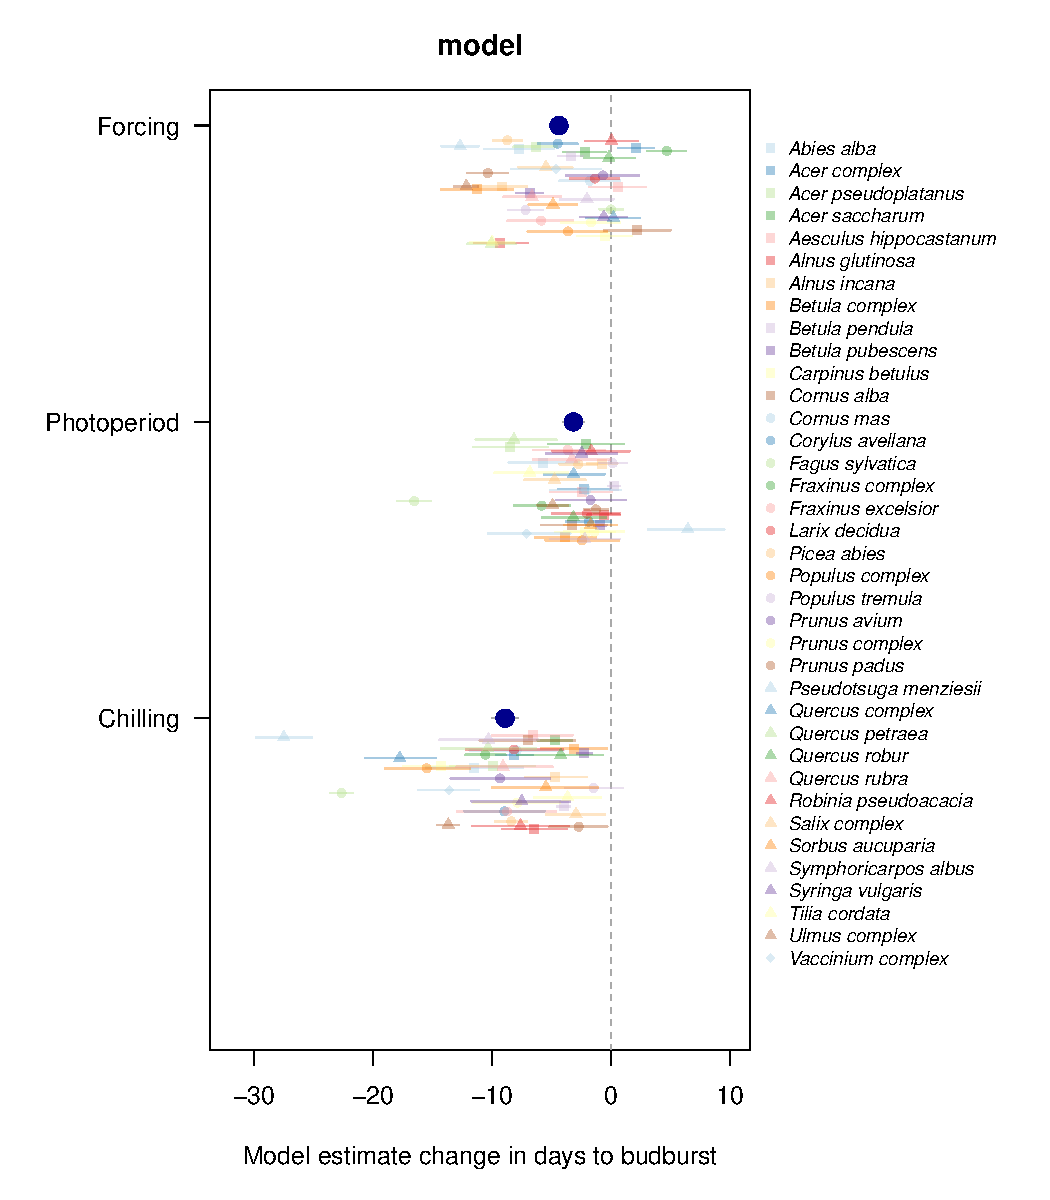
\includegraphics[width=0.75\textwidth]{..//..//analyses/bb_analysis/figures/muplotmodelspcompexprampfputah_z.pdf}
\caption{\emph{Estimates for effects of chilling exceeded forcing and photoperiod estimates} in the budburst models fit to data from the OSPREE database. Here we show estimates from the model fit to centered data, enabling comparisons of effects sizes across predictors, and using Utah units to quantify chilling. Estimates to models fit to uncentered data and using Chill Portions were qualitatively similar and can be found in the Supplemental Materials.} 
\label{fig:mu}
\end{figure}

%\begin{figure}[h!]
%\centering
%\noindent 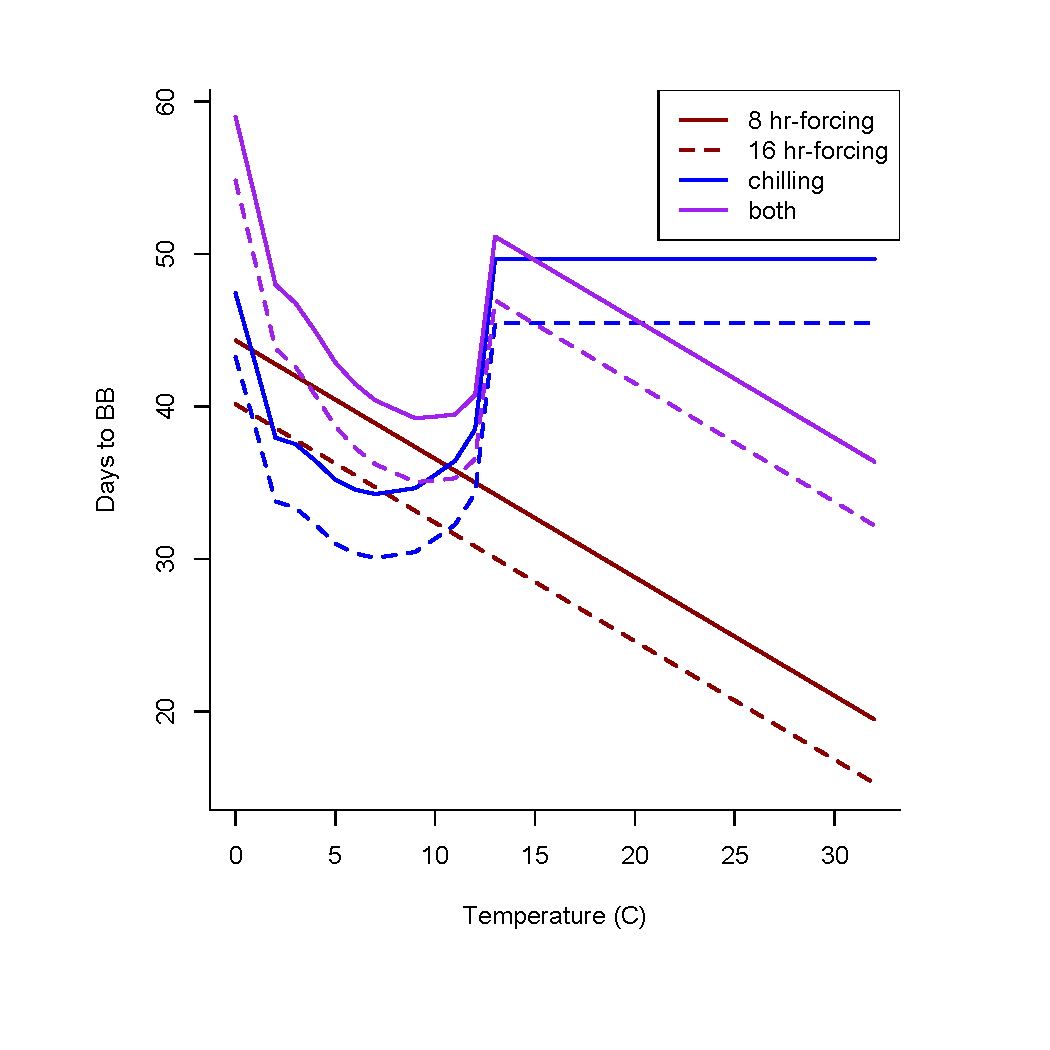
\includegraphics[width=0.75\textwidth]{..//..//analyses/bb_analysis/figures/expcondi_forecastplot.pdf}
%\caption{Effects of chilling, forcing, and photoperiod, across the experimental conditions in the OSPREE database. make this part of a 2-panel figure with \ref{fig:mu}.}
%\label{fig:apc}
%\end{figure}
\newpage
\begin{figure}[h!]
\centering
\noindent 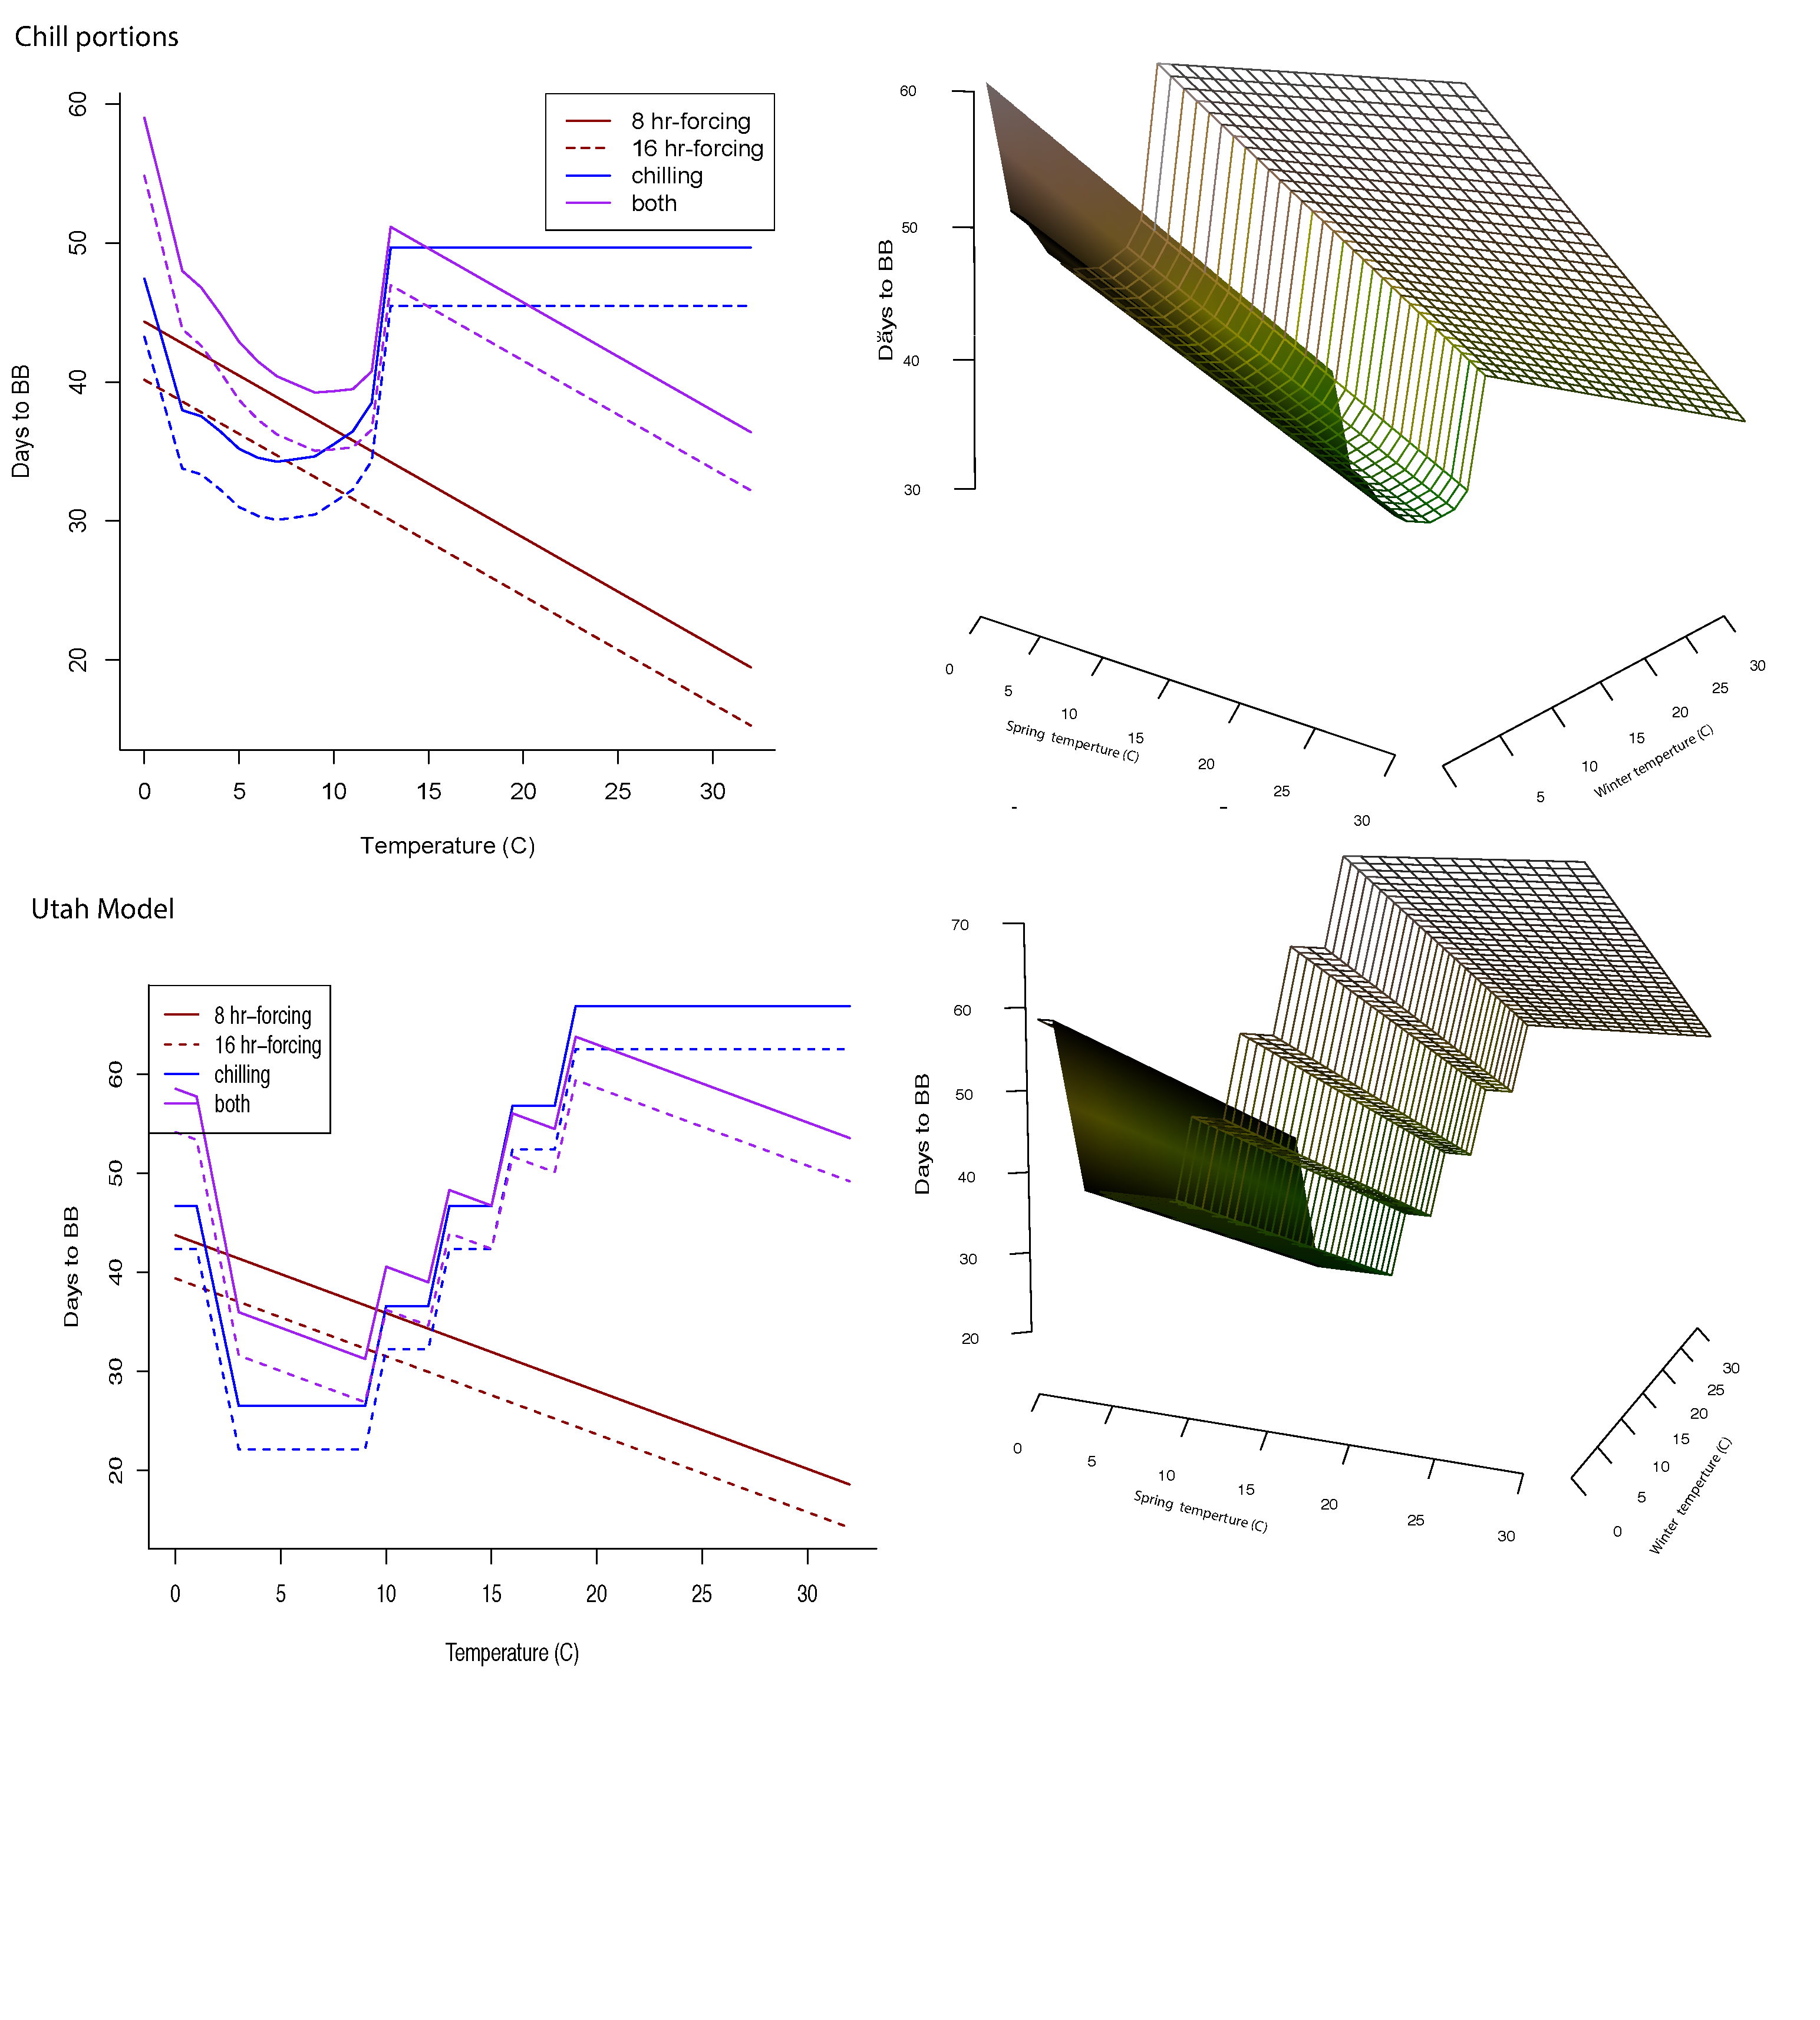
\includegraphics[width=0.75\textwidth]{..//..//analyses/bb_analysis/figures/bbmod_3dplot_4panels.pdf}
\caption{Effects of chilling, forcing, and photoperiod, across the experimental conditions in the OSPREE database. Make this part of a 2-panel figure with \ref{fig:mu}?}
\label{fig:apc}
\end{figure}


\newpage

\begin{figure}[h!]
\centering
\noindent 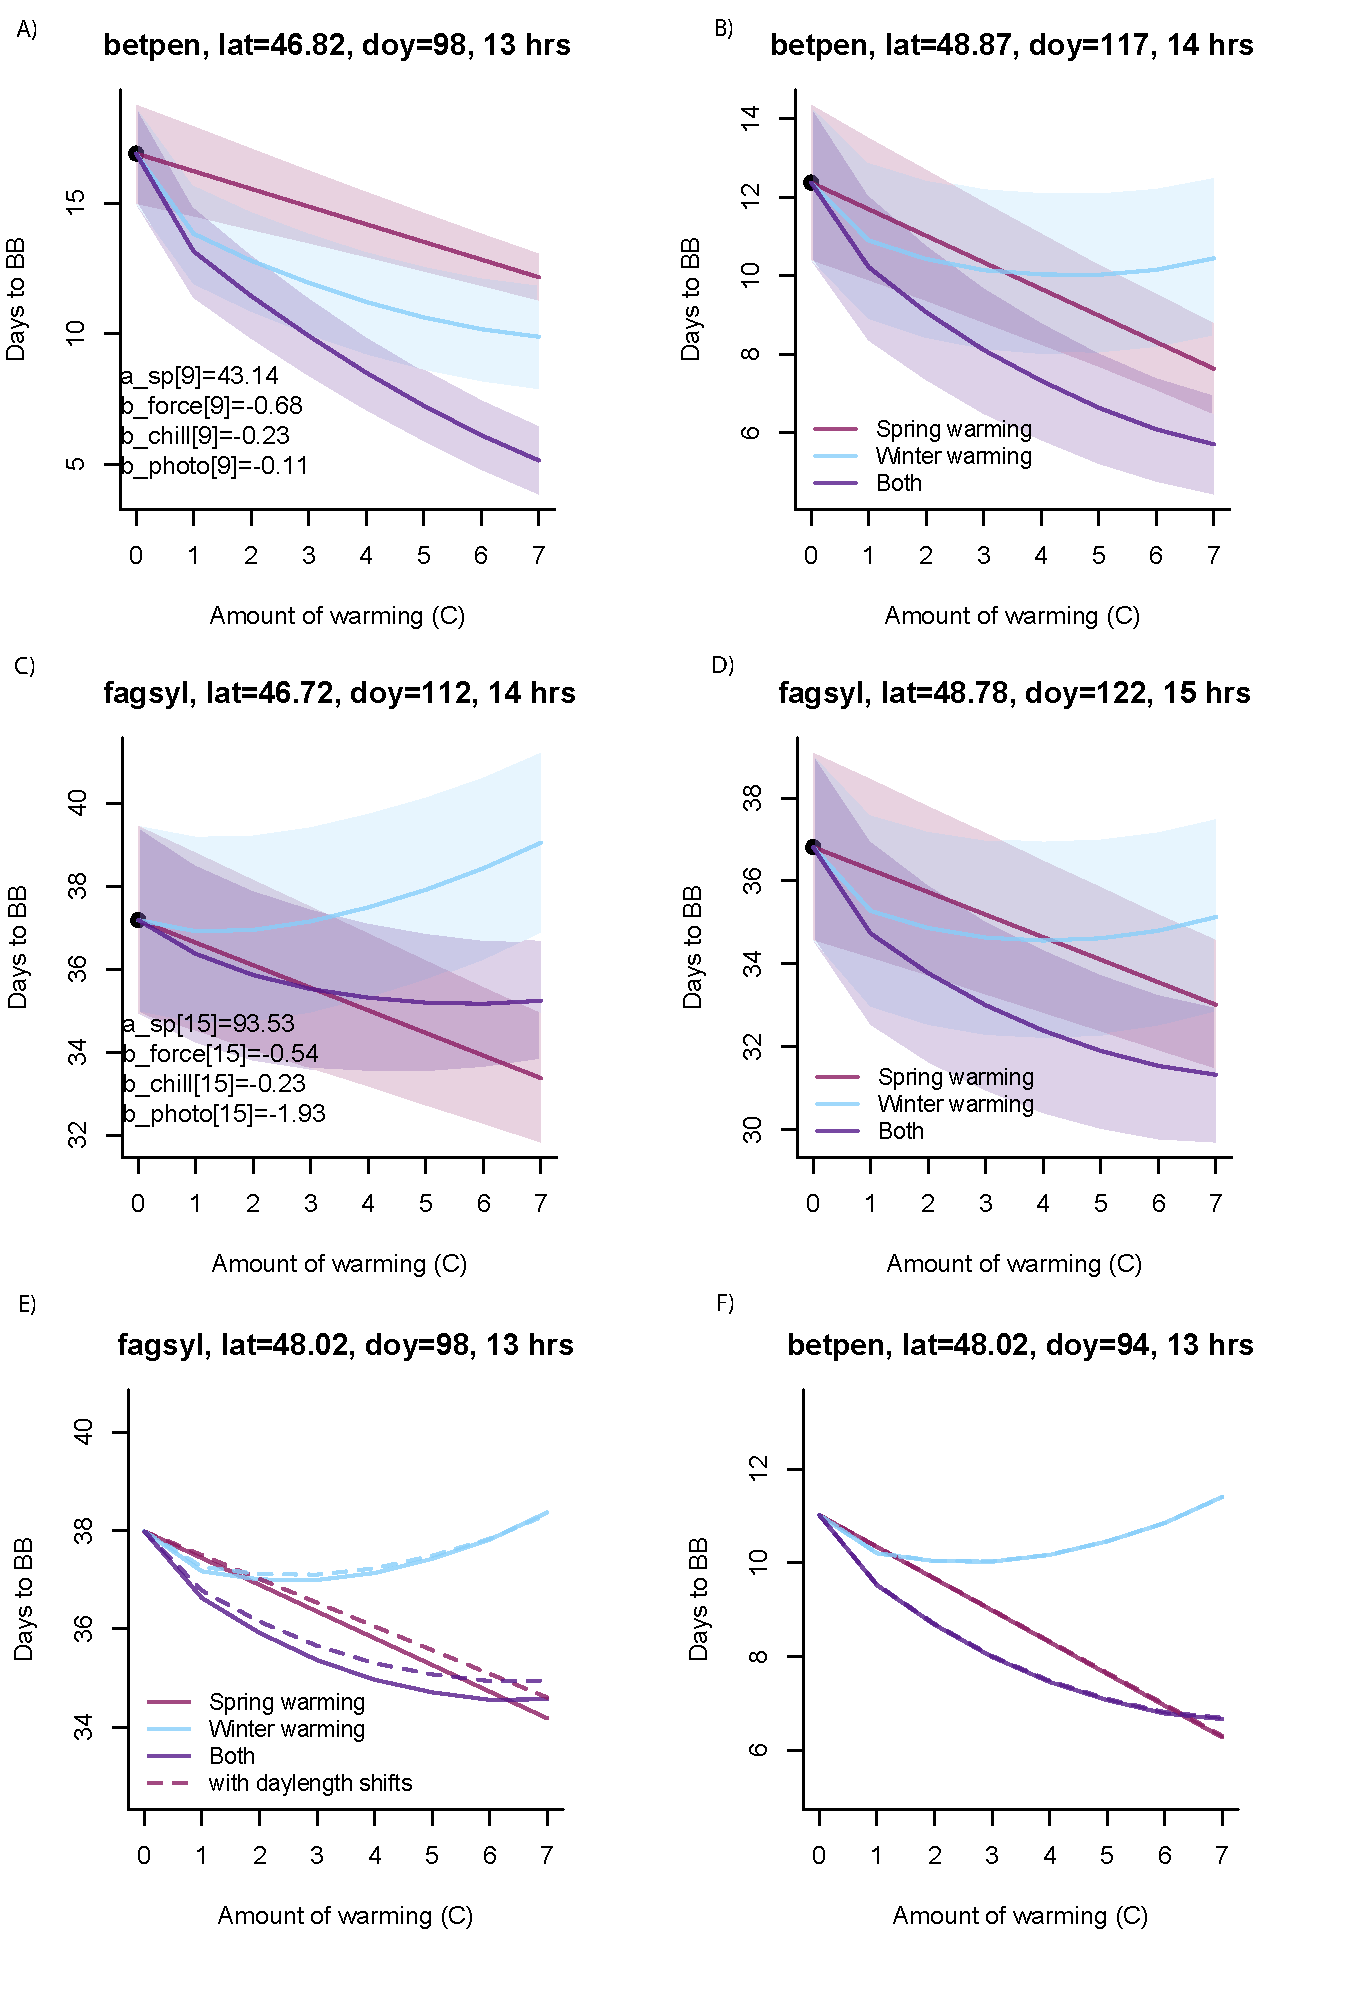
\includegraphics[width=0.75\textwidth]{..//..//analyses/bb_analysis/figures/forecasting/tempforecast_betpenfagsyl_minmaxlat_PEPBB_wdl.pdf}
\caption{Implications of global warming on budburst of \emph{Betula pendula} (A,B) and \emph{Fagus sylvatica} (C,D) as predicted by the OSPREE model. We show the maximum and minimum latitudes at which each species occurred in the PEP database for Germany as examples; these locations differ in current climate. For all sites effects of potential shifts in photoperiod with advancing budbrst were minimal (E,F), even the photosensitive species \emph{Fagus sylvatica}}%Species forecasting with PEP data: \emph{Betula, Fagus} ... need to think on which ones to use (x sites x species focus etc). ... Maybe show photoperiod one?

\label{fig:fore}
\end{figure}

\newpage
\begin{figure}[h!]
\centering
\noindent 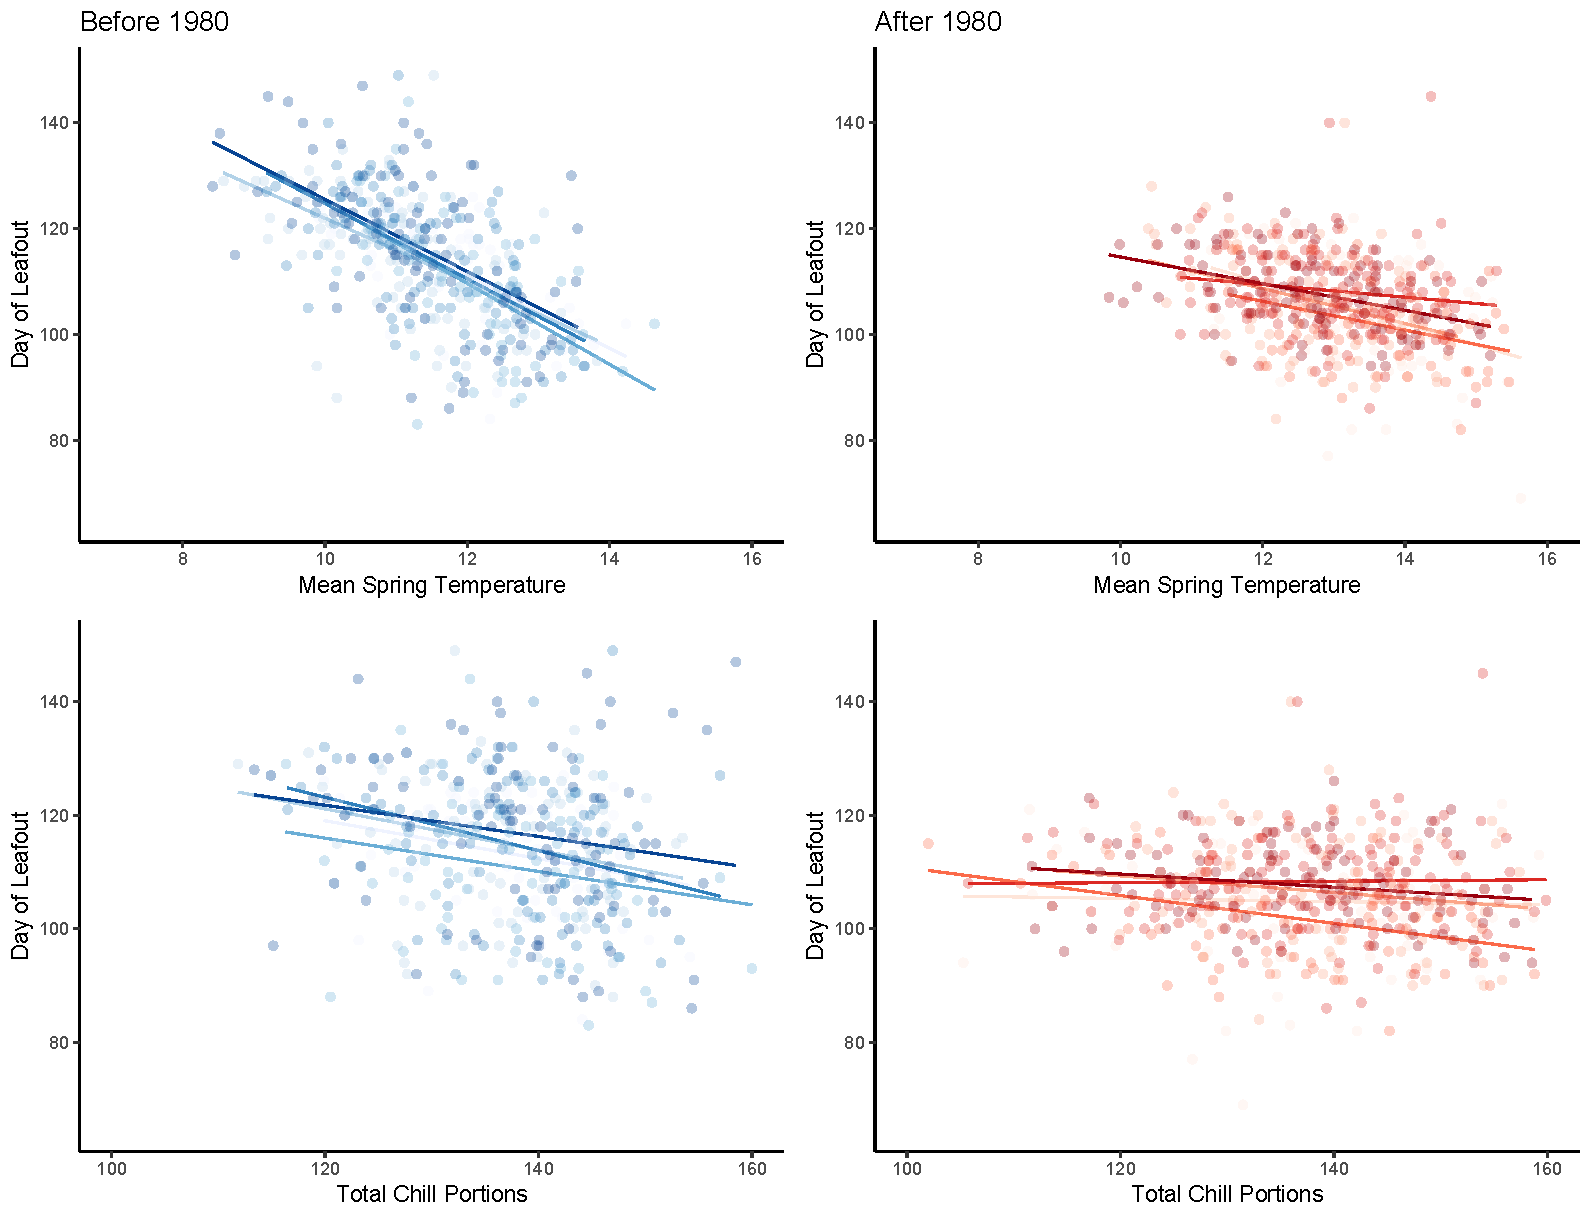
\includegraphics[width=0.75\textwidth]{..//..//analyses/bb_analysis/PEP_climate/figures/BETPEN_multruns_portions.pdf}
\caption{Implications of global warming on budburst of \emph{Betula pendula} (A,B) and \emph{Fagus sylvatica} (C,D) as predicted by the OSPREE model. We show the maximum and minimum latitudes at which each species occurred in the PEP database for Germany as examples; these locations differ in current climate. For all sites effects of potential shifts in photoperiod with advancing budbrst were minimal (E,F), even the photosensitive species \emph{Fagus sylvatica}}
\label{fig:pep}
\end{figure}


\section*{Reference list}

A few categories:\\

Papers about contrasting results over what cues matter from growth chamber studies: \cite{Basler:2012,Basler:2014aa,Caffarra:2011qf,Caffarra:2011a,Caffarra:2011b,Heide:2005aa,koerner2010b,Laube:2014a,vitasse2013,zohner2016}. Get Nanninga \emph{et al.} 2017: 'Increased exposure to chilling advances the time to budburst in North American tree species' and maybe Malyshev \emph{et al.} 2018 `Temporal photoperiod sensitivity and forcing requirements for budburst in temperate tree seedlings.'\\

Papers about declining sensitivities: \cite{Rutishauser:2008,fu2015}. Also look for a Wang \emph{et al.} article `Impacts of global warming on phenology of spring leaf unfolding remain stable in the long run.' Vitasse paper on declining variation across elevation gradient. See \cite{yu2010}, but this is not temperate trees. \\

Papers about chilling units paper (Lizzie gets a list): Fu 2012 from OSPREE. \cite{harrington2015}\cite{lued2011,Luedeling:2011qe,Luedeling2013AgFM}\\

\bibliography{..//..//refs/ospreebibplus.bib}

%%%%%%%%%%%%%%%%%%%%%%%%%%%%%%%%%%%%%%%%
\end{document}
%%%%%%%%%%%%%%%%%%%%%%%%%%%%%%%%%%%%%%%%
